\section{Resultados Nº Envoltório}
\subsection{Diâmetro 2}

\begin{frame}
\frametitle{Estudos teóricos dissertação}
\framesubtitle{diâmetro 2}
\begin{columns}[T]
 \begin{column}{.5\textwidth}
Número envoltório e Carathéodory em Grafos Diâmetro 2:
\begin{enumerate}
\item{Geral}
\item{Maximal Sem Triângulo}
\item{Fortemente Regular}
\end{enumerate}
\end{column}
\begin{column}{.5\textwidth}
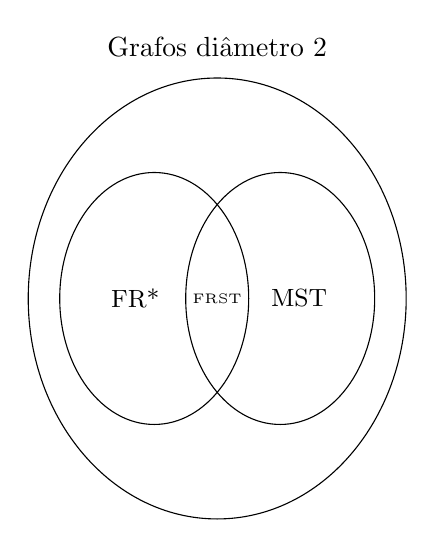
\begin{tikzpicture}[scale=0.8]
\draw  (-2,2) ellipse (1.5 and 2);
\draw  (0,2) ellipse (1.5 and 2);
\draw  (-1,2) ellipse (3 and 3.5);
\node at (-1,2) {\tiny FRST};
\node at (-1,6) {Grafos diâmetro 2};
\node at (-2.3,2) {\small FR*};
\node at (0.3,2) {\small MST};
\end{tikzpicture}
\end{column}
\end{columns}
\end{frame}


\begin{frame}
\frametitle{Nº Envoltório}
\framesubtitle{diâmetro 2}
 \begin{columns}[T]
     \begin{column}{.6\textwidth}
    \begin{proposition}
    Seja $G$ um grafo de diâmetro 2:
    \begin{enumerate}
    \label{prop:diametro2}
    \item{Para todo $u,v \in V(G)$, $u$ e $v$ são adjacentes ou tem um vizinho em comum} \label{pro-diam-2-itema}
    \item{$N(v)$ é um conjunto dominante $\forall v \in V(G)$} \label{pro-diam-2-itemb}
    \item Se $v \in V(G)$ é um vértice de corte então $d(v)=n-1$\label{pro-diam-2-itemd}
    \item{Se $G$ tem vértice de corte então $\Delta(G)=n-1$}\label{pro-diam-2-iteme}
    \item Existe no máximo um vértice de corte em $G$\label{pro-diam-2-itemf}
    \end{enumerate}
    \end{proposition}
    \end{column}
 
    \begin{column}{.4\textwidth}
    \centering
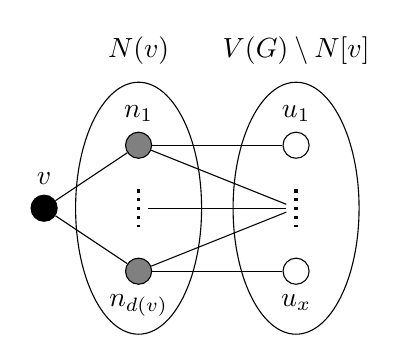
\begin{tikzpicture}[scale=0.8]
    \draw  (0,0) ellipse (1 and 2);
    \node[circle,draw,label=$v$,fill] (v1) at (-1.5,0) {};
    \node[circle,draw,label=$n_{1}$,fill=black!50] (v2) at (0,1) {};
    \node[circle,draw,label=below:$n_{d(v)}$,fill=black!50] (v3) at (0,-1) {};
    \draw [very thick,dotted] (0,0.3) -- (0,-0.3);

    \node (v7) at (0,0) {};

    \draw  (v1) edge (v2);
    \draw  (v1) edge (v3);

    \node at (0,2.5) {$N(v)$};

    \draw  (2.5,0) ellipse (1 and 2);
    \node at (2.5,2.5) {$V(G) \setminus N[v]$};

    \node[circle,draw,label=$u_1$] (v4) at (2.5,1) {};
    \node (v5) at (2.5,0) {};
    \draw [very thick,dotted] (2.5,0.3) -- (2.5,-0.3);
    \node[circle,draw,label=below:$u_x$] (v6) at (2.5,-1) {};

    \draw  (v2) edge (v5);
    \draw  (v2) edge (v4);
    \draw  (v3) edge (v6);
    \draw  (v3) edge (v5);
    \draw  (v7) edge (v5);
\end{tikzpicture}
    \end{column}

  \end{columns}
\end{frame}



\begin{frame}
\frametitle{Nº Envoltório}
\framesubtitle{diâmetro 2 - com vértice de corte}
\begin{columns}[T]
 \begin{column}{.5\textwidth}

\begin{proposition}
    Se $G$ é um grafo de diâmetro 2 com vértice de corte $v$ então $h(G) \leq \omega(G-v)$. 
\end{proposition}

\end{column}
\begin{column}{.5\textwidth}
\centering
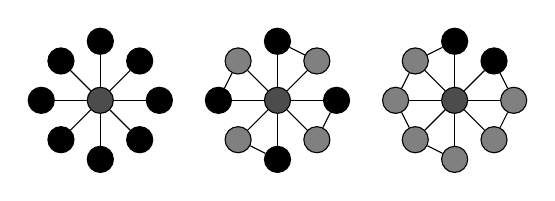
\begin{tikzpicture}[scale=0.5]
\node[circle,draw,fill=black!70] (v1) at (-13.5,-1) {};
\node[circle,draw,fill] (v3) at (-13.5,0.5) {};
\node[circle,draw,fill] (v9) at (-15,-1) {};
\node[circle,draw,fill] (v7) at (-13.5,-2.5) {};
\node[circle,draw,fill] (v5) at (-12,-1) {};
\node[circle,draw,fill] (v8) at (-14.5,-2) {};
\node[circle,draw,fill] (v6) at (-12.5,-2) {};
\node[circle,draw,fill] (v4) at (-12.5,0) {};
\node[circle,draw,fill] (v2) at (-14.5,0) {};
\draw  (v1) edge (v2);
\draw  (v1) edge (v3);
\draw  (v1) edge (v4);
\draw  (v1) edge (v5);
\draw  (v1) edge (v6);
\draw  (v7) edge (v1);
\draw  (v1) edge (v8);
\draw  (v1) edge (v9);

\node[circle,draw,fill=black!70] (v31) at (-9,-1) {};
\node[circle,draw,fill] (v33) at (-9,0.5) {};
\node[circle,draw,fill] (v39) at (-10.5,-1) {};
\node[circle,draw,fill] (v37) at (-9,-2.5) {};
\node[circle,draw,fill] (v35) at (-7.5,-1) {};
\node[circle,draw,fill=black!50] (v38) at (-10,-2) {};
\node[circle,draw,fill=black!50] (v36) at (-8,-2) {};
\node[circle,draw,fill=black!50] (v34) at (-8,0) {};
\node[circle,draw,fill=black!50] (v32) at (-10,0) {};
\draw  (v31) edge (v32);
\draw  (v31) edge (v33);
\draw  (v31) edge (v34);
\draw  (v31) edge (v35);
\draw  (v31) edge (v36);
\draw  (v37) edge (v31);
\draw  (v31) edge (v38);
\draw  (v31) edge (v39);

\node[circle,draw,fill=black!70] (v21) at (-4.5,-1) {};
\node[circle,draw,fill] (v23) at (-4.5,0.5) {};
\node[circle,draw,fill=black!50] (v29) at (-6,-1) {};
\node[circle,draw,fill=black!50] (v27) at (-4.5,-2.5) {};
\node[circle,draw,fill=black!50] (v25) at (-3,-1) {};
\node[circle,draw,fill=black!50] (v28) at (-5.5,-2) {};
\node[circle,draw,fill=black!50] (v26) at (-3.5,-2) {};
\node[circle,draw,fill] (v24) at (-3.5,0) {};
\node[circle,draw,fill=black!50] (v22) at (-5.5,0) {};
\draw  (v21) edge (v22);
\draw  (v21) edge (v23);
\draw  (v21) edge (v24);
\draw  (v21) edge (v25);
\draw  (v21) edge (v26);
\draw  (v27) edge (v21);
\draw  (v21) edge (v28);
\draw  (v21) edge (v29);
\draw  (v24) edge (v25);
\draw  (v26) edge (v25);
\draw  (v28) edge (v29);
\draw  (v28) edge (v27);
\draw  (v22) edge (v29);
\draw  (v23) edge (v22);

\draw  (v34) edge (v33);
\draw  (v36) edge (v35);
\draw  (v37) edge (v38);
\draw  (v39) edge (v32);
\end{tikzpicture}
\end{column}
\end{columns}
\end{frame}



\begin{frame}
\frametitle{Nº Envoltório}
\framesubtitle{diâmetro 2 - sem vértice de corte}
% \begin{columns}[T]
% \begin{column}{.6\textwidth}
\begin{lem}
     \label{hs-dominante-envoltorio}
     Seja $G$ um grafo de diâmetro 2 sem vértice de corte e $S^\prime \subseteq V(G)$. Se $H(S^\prime)$ é um conjunto dominante, logo $G$ possui um conjunto envoltório $S$ tal que  $S=S^\prime \cup \{v\}$ para todo $v\in V(G) \setminus H(S^\prime)$.
\end{lem}
Demonstração:
\begin{itemize}
    \item Direta 
    \item Contradição
\end{itemize}

% \end{column}
% \begin{column}{.4\textwidth}
\centering
%\begin{tikzpicture}[scale=0.8]
%\node (v1) at (-12.0729,6.5067) {};
%\node (v5) at (-12.0729,5.5067) {};  
%\node[draw,circle,inner sep=0pt,minimum size=5pt,label=right:$v$] (v) at (-10.3012,6.8026) {};
%\node[draw,circle,inner sep=0pt,minimum size=5pt,label=right:$u$] (u) at (-10.2191,5.2937) {};
%\node[draw,ellipse,minimum width=1.5cm,minimum height=2.5cm,label={\scriptsize $H(S^\prime)$}] (v6) at (-11.9,6) {};
%\node[draw,ellipse,minimum width=1.5cm,minimum height=2.5cm,label={\scriptsize $V(G) \setminus H(S^\prime)$}] at (-10.1,6) {};
%\draw  (v1) edge (v);
%\draw  (v5) edge (u);
%\draw  (v) edge (u);
%\node[draw,circle,inner sep=0pt,minimum size=5pt,label=right:$v$] (vc) at (-12.4,2.8) {};
%\node[draw,circle,inner sep=0pt,minimum size=5pt,label=right:$u$] (uc) at (-12.4,1) {};
%\node[draw,ellipse,minimum width=1.5cm,minimum height=2.5cm,label={\scriptsize $H(S^\prime)$}] at (-14,2) {};
%        \node[draw,ellipse,minimum width=1.5cm,minimum height=2.5cm,label={\scriptsize $V(G) \setminus H(S^\prime)$}] at (-12.2,2) {};
%        \node[draw,circle,inner sep=0pt,minimum size=5pt,label=right:$w^\prime$] (v4) at (-12.5,2) {};
%        \draw  (uc) edge (v4);
%        \draw  (v4) edge (vc);
%        \node (v9) at (-14,2.5) {};
%        \node (v10) at (-14,1.5) {};
%        \node[draw,circle,inner sep=0pt,minimum size=5pt,label=right:$v$] (vc2) at (-8.5,3) {};
%        \node[draw,circle,inner sep=0pt,minimum size=5pt,label=right:$u$] (uc2) at (-8.5,1) {};
%        \node[draw,circle,inner sep=0pt,minimum size=5pt,label=right:$w$] (wc2) at (-10,2) {};
%        \node[draw,ellipse,minimum width=1.5cm,minimum height=2.5cm,label={\scriptsize $H(S^\prime)$}] at (-10.1,2) {};
%        \node[draw,ellipse,minimum width=1.5cm,minimum height=2.5cm,label={\scriptsize $V(G) \setminus H(S^\prime)$}] at (-8.4,2) {};
%        \node at (-10.2,2.7) {};
%        \node at (-10.1,1.5) {};
%        \draw  (vc2) edge (wc2);
%        \draw  (uc2) edge (wc2);
%        \node at (-11,4.5) {\tiny Caso 1};
%        \node at (-13.1,0.5) {\tiny Caso 2a};
%        \node at (-9.2,0.5) {\tiny Caso 2b};
%        \draw  (v9) edge (vc);
%        \draw  (uc) edge (v10);
%        \draw[snake=zigzag,dashed]  (vc2) edge (uc2);
%        \node at (-8,2) {$P_{vu}$};
%    \end{tikzpicture}
%    \end{column}
%  \end{columns}
\end{frame}

\begin{frame}
\frametitle{Nº Envoltório}
\framesubtitle{diâmetro 2 - sem vértice de corte}
\begin{columns}[T]
\begin{column}{.6\textwidth}
 \begin{coro}
  Se $G$ é um grafo de diâmetro 2 sem vértice de corte então $h(G) \le \delta + 1$.
 \end{coro}
 \begin{coro} Se $G$ é um grafo de diâmetro 2, então $h(G) \le  \sqrt{n\ln(n)} + 2$.
\label{coro-domina1}
\end{coro}

\begin{coro}
\label{coro-domina2}
Seja $G$ um grafo de diâmetro 2 sem vértice de corte. Se $\delta \ge \sqrt[]{n}ln(n)$ então $h(G) \le \sqrt[]{n} + 2$.
\end{coro}
\end{column}
\begin{column}{.4\textwidth}
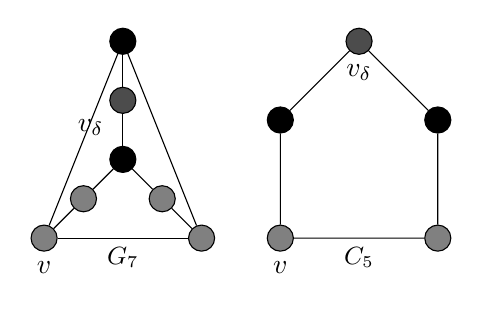
\begin{tikzpicture}[scale=0.5]
  \node[circle,draw,fill=black!70,label=below left:$v_\delta$] (v1) at (-6,3.5) {};
  \node[circle,draw,fill] (v3) at (-6,2) {};
  \node[circle,draw,fill=black!50] (v4) at (-7,1) {};
  \node[circle,draw,fill=black!50] (v5) at (-5,1) {};
  \node[circle,draw,fill=black!50] (v6) at (-4,0) {};
  \node[circle,draw,fill=black!50,label=below:$v$] (v7) at (-8,0) {};
  \node[circle,draw,fill] (v8) at (-6,5) {};

  \draw  (v8) edge (v1);
  \draw  (v1) edge (v3);
  \draw  (v3) edge (v4);
  \draw  (v3) edge (v5);
  \draw  (v5) edge (v6);
  \draw  (v7) edge (v4);
  \draw  (v7) edge (v8);
  \draw  (v8) edge (v6);
  \draw  (v7) edge (v6);
  
  \node[circle,draw,fill=black!70,label=below:$v_\delta$] (v9) at (0,5) {};
  \node[circle,draw,fill] (v10) at (2,3) {};
  \node[circle,draw,fill=black!50] (v11) at (2,0) {};
  \node[circle,draw,fill=black!50,label=below:$v$] (v12) at (-2,0) {};
  \node[circle,draw,fill] (v13) at (-2,3) {};
  
  \draw (v9) -- (v10) -- (v11) -- (v12) -- (v13) -- (v9);
  
  \node at (-6,-0.5) {\small $G_7$};
  \node at (0,-0.5) {\small $C_5$};
\end{tikzpicture}
\end{column}
\end{columns}
\end{frame}


\begin{frame}
\frametitle{Nº Envoltório}
\framesubtitle{diâmetro 2 - sem vértice de corte}
\centering
\textbf{Melhorando Limite com Algoritmo}
\end{frame}


\begin{frame}
\frametitle{Nº Envoltório}
\framesubtitle{diâmetro 2 - sem vértice de corte}
\begin{columns}[T]
\begin{column}{.5\textwidth}
Seja $G$ um grafo de diâmetro 2 e $C\subseteq V(G)$ não vazio:
\begin{enumerate}
\item {Conjunto N: subconjunto de $V(G)\setminus C$ contendo todos os vértices que são adjacentes a algum vértice de $C$, mas que não pertença a $C$, ou seja $N=N(C)\setminus C$}
\item {Conjunto $O$: subconjunto de $V(G)\setminus N[C]$ contendo os vértices que são adjacentes somente a vértice de $N$, ou seja $O= N[N] \setminus N[C]$}
\item {$V(G)= C \cup N \cup O$}
\end{enumerate}
\end{column}
\begin{column}{.5\textwidth}
\centering
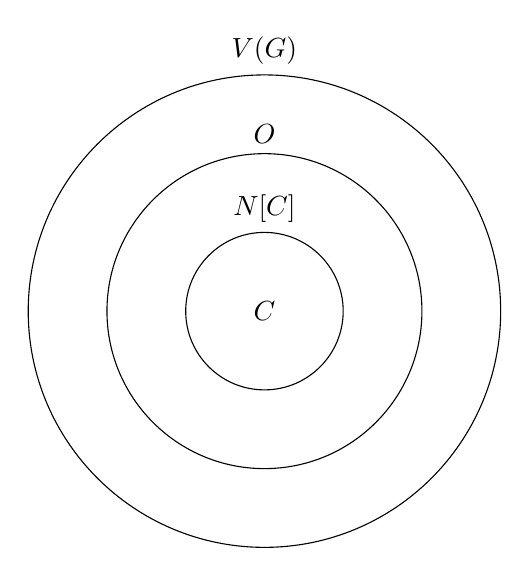
\begin{tikzpicture}[scale=0.8]
  \node[draw,circle,minimum size=2cm,label={$N[C]$}] (c) at (0, 0) { $C$ };
  \node[draw,circle,minimum size=4cm,label={$O$}] (nc) at (0, 0) {};
  \node[draw,circle,minimum size=6cm,label={$V(G)$}] (ext) at (0, 0) {};
\end{tikzpicture}
\end{column}
\end{columns}
\end{frame}


\begin{frame}
\frametitle{Nº Envoltório}
\framesubtitle{diâmetro 2  - sem vértice de corte}
\begin{columns}[T]
\begin{column}{.5\textwidth}
\begin{proposition}
Seja $G$ um grafo de diâmetro 2 e $S \subseteq V(G)$. Considere $C=H(S)$, $N=N(C) \setminus C$ e $O=V(G) \setminus N[C]$ então:
\begin{enumerate}
\item{Se $O$ é vazio então $H(S)$ é dominante} 
\item{Se $o \in O$ então $d(o) \ge |H(S)|$}
\item{Se $|H(S)| > \Delta$ então $O$ é vazio}
\end{enumerate}
\end{proposition}
\end{column}
\begin{column}{.5\textwidth}
\centering
\resizebox{\textwidth}{!}{%
\centering
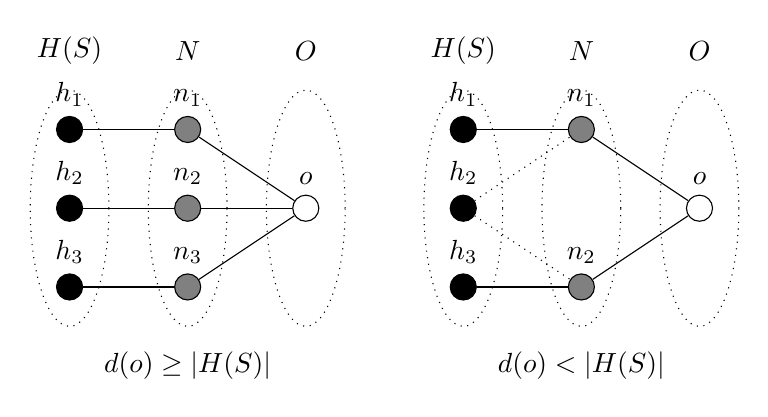
\begin{tikzpicture}
\node[circle,draw,fill,label=$h_1$] (v1) at (-5,2.5) {};
\node[circle,draw,fill,label=$h_2$] (v3) at (-5,1.5) {};
\node[circle,draw,fill,label=$h_3$] (v5) at (-5,0.5) {};
\node[circle,draw,fill,fill=black!50,label=$n_1$] (v2) at (-3.5,2.5) {};
\node[circle,draw,fill,fill=black!50,label=$n_2$] (v4) at (-3.5,1.5) {};
\node[circle,draw,fill,fill=black!50,label=$n_3$] (v6) at (-3.5,0.5) {};
\node[circle,draw,label=$o$] (v7) at (-2,1.5) {};

\node[circle,draw,fill,label=$h_1$] (v9) at (0,2.5) {};
\node[circle,draw,fill,label=$h_2$] (v13) at (0,1.5) {};
\node[circle,draw,fill,label=$h_3$] (v10) at (0,0.5) {};
\node[circle,draw,fill,fill=black!50,label=$n_1$] (v8) at (1.5,2.5) {};
\node[circle,draw,fill,fill=black!50,label=$n_2$] (v11) at (1.5,0.5) {};
\node[circle,draw,label=$o$] (v12) at (3,1.5) {};

\draw  (v1) edge (v2);
\draw  (v3) edge (v4);
\draw  (v5) edge (v6);
\draw  (v2) edge (v7);
\draw  (v4) edge (v7);
\draw  (v6) edge (v7);
\draw  (v8) edge (v9);
\draw  (v10) edge (v11);
\draw  (v8) edge (v12);
\draw  (v11) edge (v12);
\draw[dotted]  (v13) edge (v11);
\draw[dotted]  (v13) edge (v8);

\node at (-5,3.5) {$H(S)$};
\node at (-3.5,3.5) {$N$};
\node at (-2,3.5) {$O$};
\node at (0,3.5) {$H(S)$};
\node at (1.5,3.5) {$N$};
\node at (3,3.5) {$O$};

\node at (-3.5,-0.5) {$d(o)\ge|H(S)|$};
\node at (1.5,-0.5) {$d(o)<|H(S)|$};

\draw[dotted]  (-5,1.5) ellipse (0.5 and 1.5);
\draw[dotted]  (3,1.5) ellipse (0.5 and 1.5);
\draw[dotted]  (1.5,1.5) ellipse (0.5 and 1.5);
\draw[dotted]  (0,1.5) ellipse (0.5 and 1.5);
\draw[dotted]  (-2,1.5) ellipse (0.5 and 1.5);
\draw[dotted]  (-3.5,1.5) ellipse (0.5 and 1.5);
\end{tikzpicture}
}
\end{column}
\end{columns}
\end{frame}


\begin{frame}
\frametitle{Nº Envoltório}
\framesubtitle{diâmetro 2 - sem vértice de corte}
  \begin{columns}[T]
    \begin{column}{.5\textwidth}
    \begin{algorithm}[H]
    \SetAlFnt{\tiny}
    \SetAlCapFnt{\small}
    \SetAlCapNameFnt{\small}
    \SetAlgoLined
    \DontPrintSemicolon
    \LinesNumbered
    \SetAlgoLined
    \BlankLine
    \Entrada{$G(V,E)$}
    \Saida{$S^\prime$ tal que $N(H(S^\prime)) = V(G)$}
    \BlankLine

    %$i \gets 0 $\\
    $S^\prime \gets \emptyset$ \\
    $N \gets \emptyset$ \\
    $O \gets V$ \\
    \Enqto{$O \ne \emptyset$}{
         $v \gets v\in O $\\
         %$i \gets i + 1 $\\         
         $S^\prime \gets S^\prime \cup \{ v \}$\\
         $H \gets H(S^\prime)$ \\
         $N \gets N(H) \setminus H$ \\
         %$N \gets N[H]$ \\
		 $O \gets V \setminus N \cup H$ \\
    }
    \Retorna{$S^\prime$}    
    \caption{$ConjuntoFechoDominante(G(V,E))$}
    \end{algorithm}
    \end{column}
    \begin{column}{.5\textwidth}
        \begin{itemize}
            \item{Constrói um conjunto $S\prime$ cujo envoltória é dominante}
            \item{A cada iteração escolhe um novo vértice para $S\prime$}
            \item{A cada iteração $H$ dobra sua cardinalidade}
        \end{itemize}
     \end{column}
  \end{columns}
\end{frame}

\begin{frame}
\frametitle{Nº Envoltório}
\framesubtitle{diâmetro 2 - sem vértice de corte}
\centering
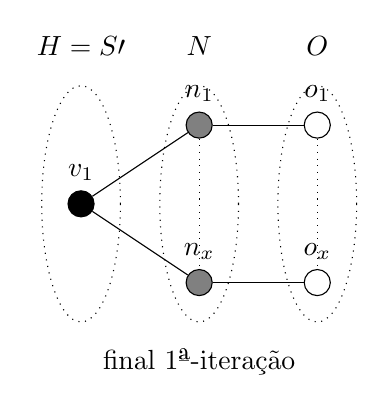
\begin{tikzpicture}
\node[circle,draw,label=$o_1$] (v1) at (-2,2.5) {};
\node[circle,draw,label=$o_x$] (v3) at (-2,0.5) {};
\node[circle,draw,fill,fill=black!50,label=$n_1$] (v2) at (-3.5,2.5) {};
\node[circle,draw,fill,fill=black!50,label=$n_x$] (v4) at (-3.5,0.5) {};
\node[circle,draw,label=$v_1$,fill] (v7) at (-5,1.5) {};

\draw  (v1) edge (v2);
\draw  (v3) edge (v4);
\draw  (v2) edge (v7);
\draw  (v4) edge (v7);
\node at (-3.5,-0.5) {final 1ª-iteração};
\draw[dotted]  (v2) edge (v4);
\draw[dotted]  (v1) edge (v3);
\draw[dotted]  (-5,1.5) ellipse (0.5 and 1.5);
\draw[dotted]  (-2,1.5) ellipse (0.5 and 1.5);
\draw[dotted]  (-3.5,1.5) ellipse (0.5 and 1.5);

\node at (-5,3.5) {$H=S\prime$};
\node at (-3.5,3.5) {$N$};
\node at (-2,3.5) {$O$};

\end{tikzpicture}
\end{frame}


\begin{frame}
\frametitle{Nº Envoltório}
\framesubtitle{diâmetro 2 - sem vértice de corte}
\centering
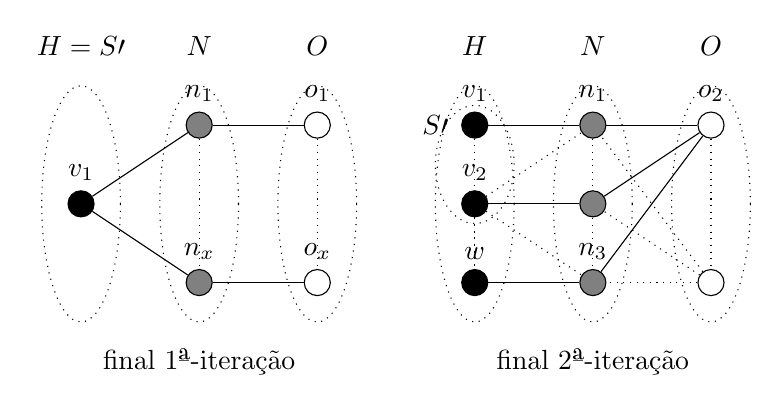
\begin{tikzpicture}
\node[circle,draw,label=$o_1$] (v1) at (-2,2.5) {};
\node[circle,draw,label=$o_x$] (v3) at (-2,0.5) {};
%\node[circle,draw,fill,label=$h_3$] (v5) at (-2,1.5) {};
\node[circle,draw,fill,fill=black!50,label=$n_1$] (v2) at (-3.5,2.5) {};
\node[circle,draw,fill,fill=black!50,label=$n_x$] (v4) at (-3.5,0.5) {};
%\node[circle,draw,fill,fill=black!50,label=$n_3$] (v6) at (-3.5,1.5) {};
\node[circle,draw,label=$v_1$,fill] (v7) at (-5,1.5) {};
\node[circle,draw,fill,label=$v_1$] (v9) at (0,2.5) {};
\node[circle,draw,fill,label=$v_2$] (v13) at (0,1.5) {};
\node[circle,draw,fill,label=$w$] (v10) at (0,0.5) {};
\node[circle,draw,fill,fill=black!50,label=$n_1$] (v8) at (1.5,2.5) {};
\node[circle,draw,fill,fill=black!50,label=$n_3$] (v11) at (1.5,0.5) {};
\node[circle,draw,label=$o_2$] (v12) at (3,2.5) {};

\draw  (v1) edge (v2);
\draw  (v3) edge (v4);
%\draw  (v5) edge (v6);
\draw  (v2) edge (v7);
\draw  (v4) edge (v7);
%\draw  (v6) edge (v7);
\draw  (v8) edge (v9);
\draw  (v10) edge (v11);
\draw  (v8) edge (v12);
\draw  (v11) edge (v12);
\draw[dotted]  (v13) edge (v11);
\draw[dotted]  (v13) edge (v8);
\node at (-5,3.5) {$H=S\prime$};
\node at (-3.5,3.5) {$N$};
\node at (-2,3.5) {$O$};
\node at (0,3.5) {$H$};
\node at (1.5,3.5) {$N$};
\node at (3,3.5) {$O$};
\draw[dotted]  (-5,1.5) ellipse (0.5 and 1.5);
\draw[dotted]  (3,1.5) ellipse (0.5 and 1.5);
\draw[dotted]  (1.5,1.5) node (v16) {} ellipse (0.5 and 1.5);
\draw[dotted]  (0,1.5) ellipse (0.5 and 1.5);
\draw[dotted]  (-2,1.5) ellipse (0.5 and 1.5);
\draw[dotted]  (-3.5,1.5) ellipse (0.5 and 1.5);
\draw[dotted]  (0,2) ellipse (0.5 and 0.75);
\draw[dotted]  (v2) edge (v4);
\node[draw,circle] (v14) at (3,0.5) {};
\draw[dotted]  (v1) edge (v3);
\draw[dotted]  (v12) edge (v14);
\draw[dotted]  (v8) edge (v11);
\node[draw,circle,fill=black!50] (v15) at (1.5,1.5) {};
\draw  (v12) edge (v15);
\draw  (v15) edge (v13);
\draw[dotted]  (v14) edge (v11);
\draw[dotted]  (v14) edge (v16);
\draw[dotted]  (v14) edge (v8);
\node at (-0.5,2.5) {$S\prime$};
\draw[dotted]  (v9) edge (v10);
\draw[dotted]  (v13) edge (v10);

\node at (-3.5,-0.5) {final 1ª-iteração};
\node at (1.5,-0.5) {final 2ª-iteração};
\end{tikzpicture}
\end{frame}


\begin{frame}
\frametitle{Nº Envoltório}
\framesubtitle{diâmetro 2 - sem vértice de corte}
\centering
\begin{columns}[T]
\begin{column}{.6\textwidth}
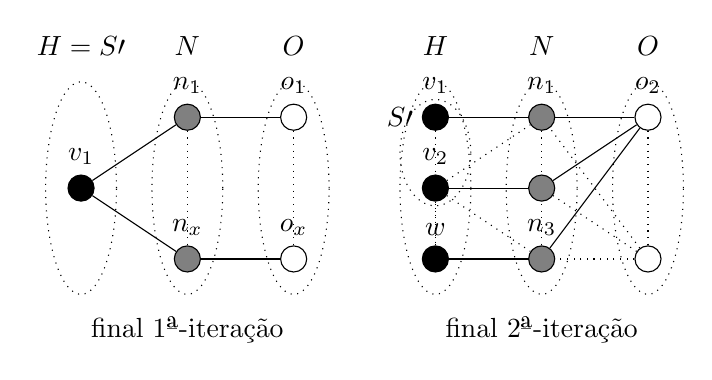
\begin{tikzpicture}[scale=0.9]
\node[circle,draw,label=$o_1$] (v1) at (-2,2.5) {};
\node[circle,draw,label=$o_x$] (v3) at (-2,0.5) {};
%\node[circle,draw,fill,label=$h_3$] (v5) at (-2,1.5) {};
\node[circle,draw,fill,fill=black!50,label=$n_1$] (v2) at (-3.5,2.5) {};
\node[circle,draw,fill,fill=black!50,label=$n_x$] (v4) at (-3.5,0.5) {};
%\node[circle,draw,fill,fill=black!50,label=$n_3$] (v6) at (-3.5,1.5) {};
\node[circle,draw,label=$v_1$,fill] (v7) at (-5,1.5) {};
\node[circle,draw,fill,label=$v_1$] (v9) at (0,2.5) {};
\node[circle,draw,fill,label=$v_2$] (v13) at (0,1.5) {};
\node[circle,draw,fill,label=$w$] (v10) at (0,0.5) {};
\node[circle,draw,fill,fill=black!50,label=$n_1$] (v8) at (1.5,2.5) {};
\node[circle,draw,fill,fill=black!50,label=$n_3$] (v11) at (1.5,0.5) {};
\node[circle,draw,label=$o_2$] (v12) at (3,2.5) {};
\draw  (v1) edge (v2);
\draw  (v3) edge (v4);
%\draw  (v5) edge (v6);
\draw  (v2) edge (v7);
\draw  (v4) edge (v7);
%\draw  (v6) edge (v7);
\draw  (v8) edge (v9);
\draw  (v10) edge (v11);
\draw  (v8) edge (v12);
\draw  (v11) edge (v12);
\draw[dotted]  (v13) edge (v11);
\draw[dotted]  (v13) edge (v8);
\node at (-5,3.5) {$H=S\prime$};
\node at (-3.5,3.5) {$N$};
\node at (-2,3.5) {$O$};
\node at (0,3.5) {$H$};
\node at (1.5,3.5) {$N$};
\node at (3,3.5) {$O$};
\draw[dotted]  (-5,1.5) ellipse (0.5 and 1.5);
\draw[dotted]  (3,1.5) ellipse (0.5 and 1.5);
\draw[dotted]  (1.5,1.5) node (v16) {} ellipse (0.5 and 1.5);
\draw[dotted]  (0,1.5) ellipse (0.5 and 1.5);
\draw[dotted]  (-2,1.5) ellipse (0.5 and 1.5);
\draw[dotted]  (-3.5,1.5) ellipse (0.5 and 1.5);
\draw[dotted]  (0,2) ellipse (0.5 and 0.75);
\draw[dotted]  (v2) edge (v4);
\node[draw,circle] (v14) at (3,0.5) {};
\draw[dotted]  (v1) edge (v3);
\draw[dotted]  (v12) edge (v14);
\draw[dotted]  (v8) edge (v11);
\node[draw,circle,fill=black!50] (v15) at (1.5,1.5) {};
\draw  (v12) edge (v15);
\draw  (v15) edge (v13);
\draw[dotted]  (v14) edge (v11);
\draw[dotted]  (v14) edge (v16);
\draw[dotted]  (v14) edge (v8);
\node at (-0.5,2.5) {$S\prime$};
\draw[dotted]  (v9) edge (v10);
\draw[dotted]  (v13) edge (v10);
\node at (-3.5,-0.5) {final 1ª-iteração};
\node at (1.5,-0.5) {final 2ª-iteração};
\end{tikzpicture}
\end{column}
\begin{column}{.4\textwidth}
\begin{lem}
Considere a i-ésima iteração do algoritmo. Se $O_i \neq \emptyset$, então $|H(S_i)|\geq 2 (|H(S_{i-1})|)+1$.
\end{lem}
\end{column}
\end{columns}
\end{frame}


\begin{frame}
\frametitle{Nº Envoltório}
\framesubtitle{diâmetro 2 - sem vértice de corte}
\begin{proposition} 
    No máximo haverá $k= \Big\lceil \lg{(\Delta(G) + 1)} \Big\rceil$ iterações.
\end{proposition}
Demonstração:
\begin{itemize}
    \item O algoritmo encerra quando $O$ é vazio e $H(S^\prime)$ for dominante
    \item No máximo quando $|H(S_i)| > \Delta$
    \item $|H(S_i)|\geq 2 (|H(S_{i-1})|)+1$
    \item $|H(S_i)|\geq 2^i-1$

\end{itemize}
\begin{coro}
Seja $G$ um grafo de diâmetro 2 sem vértice de corte então $h(G) \le \Big\lceil \lg{(\Delta(G) + 1)} \Big\rceil + 1$.
\label{coro-env-gd2}
\end{coro}
\end{frame}

\begin{frame}
\frametitle{Nº Envoltório}
\framesubtitle{diâmetro 2}
\centering
\begin{columns}[T]
\begin{column}{.4\textwidth}
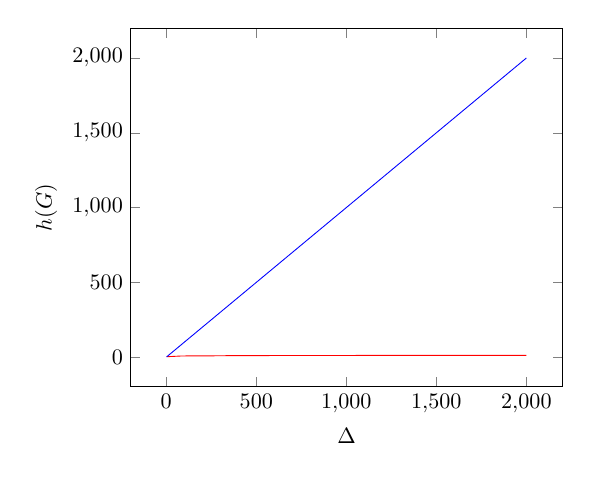
\begin{tikzpicture}[scale=0.8]
\begin{axis}[xlabel=$\Delta$,ylabel=$h(G)$]
\addplot [red,domain=2:2000]{ceil(log2(x+1))+1};
\addplot [blue,domain=2:2000]{x};
%\legend{limite}
\end{axis}
\end{tikzpicture}
\end{column}
\begin{column}{.4\textwidth}
\begin{tikzpicture}[scale=0.8]
\begin{axis}[xlabel=$\Delta$,ylabel=$h(G)$]
\addplot [red,domain=2:2000]{ceil(log2(x+1))+1};
%\addplot [blue,domain=2:2000]{x};
%\legend{$\Big\lceil \lg{(\Delta(G) + 1)} \Big\rceil + 1$}
\end{axis}
\end{tikzpicture}
\end{column}
\end{columns}
\end{frame}



\begin{frame}
\frametitle{Nº Envoltório}
\framesubtitle{diâmetro 2}
\centering
\textbf{Melhor Limite para Subclasses: Maximal sem triângulo e Fortemente regular}
\end{frame}



\subsection{Maximal Sem Triângulo}
\begin{frame}
\frametitle{Nº Envoltório}
\framesubtitle{diâmetro 2 - Maximal sem triângulo}
\begin{properties}
Grafo maximais sem triângulo:
\begin{itemize}
    \item diâmetro 2 herdando suas propriedades
    \item adição de qualquer aresta forma triângulo
    \item remoção aresta aumenta diâmetro
\end{itemize}
\end{properties}
\end{frame}

\begin{frame}
\frametitle{Nº Envoltório}
\framesubtitle{diâmetro 2 - Maximal sem triângulo}
\begin{columns}[T]
\begin{column}{.3\textwidth}
\begin{figure}
%\caption{Grafo de Petersen, $G_{pn}$}
\centering
\resizebox{\textwidth}{!}{%
    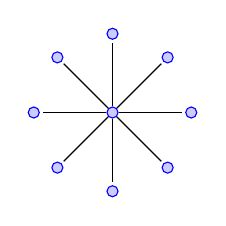
\begin{tikzpicture}[shorten >=1pt, auto, node distance=3cm,
       node_style/.style={circle,draw=blue,fill=blue!20!,inner sep=0pt, minimum width=4pt,font=\sffamily\small},
       node_style_selected/.style={circle,draw=black,fill=red!20!,font=\sffamily\Large\bfseries},
       edge_style/.style={draw=black}]
        \node[node_style] (v0) at (0,0) {};
        \node[node_style] (v1) at (0,1) {};
        \node[node_style] (v2) at (0.7,0.7) {};
        \node[node_style] (v3) at (1,0) {};
        \node[node_style] (v4) at (0.7,-0.7) {};
        \node[node_style] (v5) at (0,-1) {};
        \node[node_style] (v6) at (-0.7,-0.7) {};
        \node[node_style] (v7) at (-1,0) {};
        \node[node_style] (v8) at (-0.7,0.7) {};

        \draw[edge_style]  (v0) edge node{} (v1);
        \draw[edge_style]  (v0) edge node{} (v2);
        \draw[edge_style]  (v0) edge node{} (v3);
        \draw[edge_style]  (v0) edge node{} (v4);
        \draw[edge_style]  (v0) edge node{} (v5);
        \draw[edge_style]  (v0) edge node{} (v6);
        \draw[edge_style]  (v0) edge node{} (v7);
        \draw[edge_style]  (v0) edge node{} (v8);
    \end{tikzpicture}%
}
\end{figure}
\end{column}
\begin{column}{.3\textwidth}
\begin{figure}
%\caption{Grafo de Petersen, $G_{pn}$}
\centering
\resizebox{\textwidth}{!}{%
    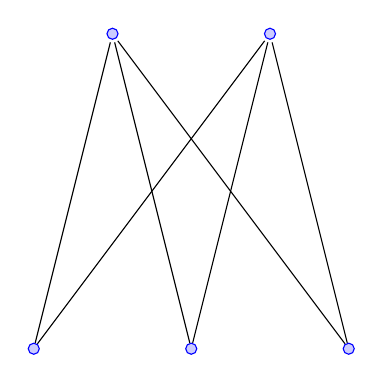
\begin{tikzpicture}[shorten >=1pt, auto, node distance=3cm,
       node_style/.style={circle,draw=blue,fill=blue!20!,inner sep=0pt, minimum width=4pt,font=\sffamily\small},
       node_style_selected/.style={circle,draw=black,fill=red!20!,font=\sffamily\Large\bfseries},
       edge_style/.style={draw=black}]
        \node[node_style] (v0) at (0,-1) {};
        \node[node_style] (v1) at (2,-1) {};
        \node[node_style] (v2) at (4,-1) {};
        \node[node_style] (v3) at (1,3) {};
        \node[node_style] (v4) at (3,3) {};

        \draw[edge_style]  (v0) edge node{} (v3);
        \draw[edge_style]  (v0) edge node{} (v4);
        \draw[edge_style]  (v1) edge node{} (v3);
        \draw[edge_style]  (v1) edge node{} (v4);
        \draw[edge_style]  (v2) edge node{} (v3);
        \draw[edge_style]  (v2) edge node{} (v4);
    \end{tikzpicture}%
}
\end{figure}
\end{column}
\begin{column}{.3\textwidth}
\begin{figure}
%\caption{Grafo de Petersen, $G_{pn}$}
\centering
\resizebox{\textwidth}{!}{%
    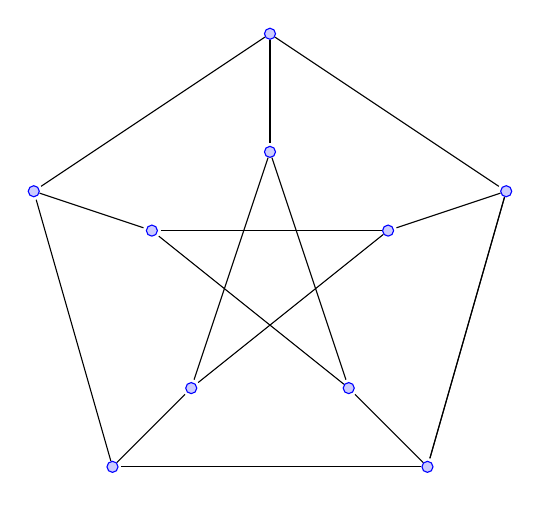
\begin{tikzpicture}[shorten >=1pt, auto, node distance=3cm,
       node_style/.style={circle,draw=blue,fill=blue!20!,inner sep=0pt, minimum width=4pt,font=\sffamily\small},
       node_style_selected/.style={circle,draw=black,fill=red!20!,font=\sffamily\Large\bfseries},
       edge_style/.style={draw=black}]
        \node[node_style] (v0) at (0,3.5) {};
        \node[node_style] (v1) at (3,1.5) {};
        \node[node_style] (v2) at (2,-2) {};
        \node[node_style] (v3) at (-2,-2) {};
        \node[node_style] (v4) at (-3,1.5) {};
        \node[node_style] (v5) at (0,2) {};
        \node[node_style] (v6) at (1.5,1) {};
        \node[node_style] (v7) at (1,-1) {};
        \node[node_style] (v8) at (-1,-1) {};
        \node[node_style] (v9) at (-1.5,1) {};

        \draw[edge_style]  (v0) edge node{} (v1);
        \draw[edge_style]  (v0) edge node{} (v4);
        \draw[edge_style]  (v0) edge node{} (v5);
        \draw[edge_style]  (v1) edge node{} (v2);
        \draw[edge_style]  (v1) edge node{} (v2);
        \draw[edge_style]  (v1) edge node{} (v6);
        \draw[edge_style]  (v2) edge node{} (v3);
        \draw[edge_style]  (v2) edge node{} (v7);
        \draw[edge_style]  (v3) edge node{} (v4);
        \draw[edge_style]  (v3) edge node{} (v8);
        \draw[edge_style]  (v4) edge node{} (v9);
        \draw[edge_style]  (v5) edge node{} (v7);
        \draw[edge_style]  (v5) edge node{} (v8);
        \draw[edge_style]  (v6) edge node{} (v8);
        \draw[edge_style]  (v6) edge node{} (v9);
        \draw[edge_style]  (v7) edge node{} (v9);
    \end{tikzpicture}%
}
\end{figure}
\end{column}
\end{columns}
\end{frame}




\begin{frame}
\frametitle{Nº Envoltório}
\framesubtitle{diâmetro 2 - Maximal Sem Triângulo}
  \begin{columns}[T]
    \begin{column}{.5\textwidth}
    \begin{proposition}
    \begin{enumerate}
        \item{Se $G$ um grafo maximal sem triângulo estrela $h(G) = n-1$} 
        \item{Seja $G$ um grafo maximal sem triângulo completo bipartido, e cada partição tem ao menos 2 vértices, então $h(G) = 2$} 
    \end{enumerate}
    \end{proposition}
    \end{column}
    \begin{column}{.2\textwidth}
        \begin{figure}
        %\caption{Grafo de Petersen, $G_{pn}$}
        \centering
        \resizebox{\textwidth}{!}{%
            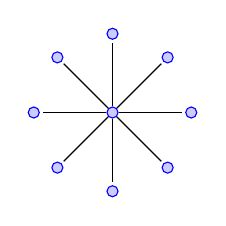
\begin{tikzpicture}[shorten >=1pt, auto, node distance=3cm,
               node_style/.style={circle,draw=blue,fill=blue!20!,inner sep=0pt, minimum width=4pt,font=\sffamily\small},
               node_style_selected/.style={circle,draw=black,fill=red!20!,font=\sffamily\Large\bfseries},
               edge_style/.style={draw=black}]
                \node[node_style] (v0) at (0,0) {};
                \node[node_style] (v1) at (0,1) {};
                \node[node_style] (v2) at (0.7,0.7) {};
                \node[node_style] (v3) at (1,0) {};
                \node[node_style] (v4) at (0.7,-0.7) {};
                \node[node_style] (v5) at (0,-1) {};
                \node[node_style] (v6) at (-0.7,-0.7) {};
                \node[node_style] (v7) at (-1,0) {};
                \node[node_style] (v8) at (-0.7,0.7) {};

                \draw[edge_style]  (v0) edge node{} (v1);
                \draw[edge_style]  (v0) edge node{} (v2);
                \draw[edge_style]  (v0) edge node{} (v3);
                \draw[edge_style]  (v0) edge node{} (v4);
                \draw[edge_style]  (v0) edge node{} (v5);
                \draw[edge_style]  (v0) edge node{} (v6);
                \draw[edge_style]  (v0) edge node{} (v7);
                \draw[edge_style]  (v0) edge node{} (v8);
            \end{tikzpicture}%
        }
        \end{figure}
    \end{column}
    \begin{column}{.2\textwidth}
        \begin{figure}
        %\caption{Grafo de Petersen, $G_{pn}$}
        \centering
        \resizebox{\textwidth}{!}{%
            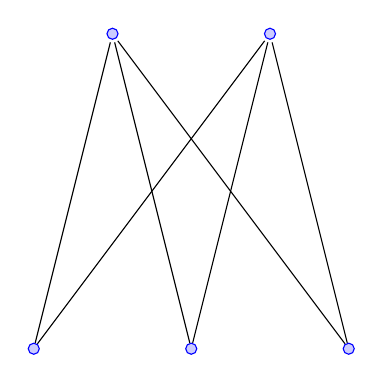
\begin{tikzpicture}[shorten >=1pt, auto, node distance=3cm,
               node_style/.style={circle,draw=blue,fill=blue!20!,inner sep=0pt, minimum width=4pt,font=\sffamily\small},
               node_style_selected/.style={circle,draw=black,fill=red!20!,font=\sffamily\Large\bfseries},
               edge_style/.style={draw=black}]
                \node[node_style] (v0) at (0,-1) {};
                \node[node_style] (v1) at (2,-1) {};
                \node[node_style] (v2) at (4,-1) {};
                \node[node_style] (v3) at (1,3) {};
                \node[node_style] (v4) at (3,3) {};

                \draw[edge_style]  (v0) edge node{} (v3);
                \draw[edge_style]  (v0) edge node{} (v4);
                \draw[edge_style]  (v1) edge node{} (v3);
                \draw[edge_style]  (v1) edge node{} (v4);
                \draw[edge_style]  (v2) edge node{} (v3);
                \draw[edge_style]  (v2) edge node{} (v4);
            \end{tikzpicture}%
        }
        \end{figure}
    \end{column}
    \end{columns}
\end{frame}


\begin{frame}
\frametitle{Nº Envoltório}
\framesubtitle{diâmetro 2 - Maximal sem triângulo  - $C_5[p, q, r, s, t]$}
  \begin{columns}[T]
    \begin{column}{.5\textwidth}
\begin{proposition}
    \begin{enumerate}
    \item{Se $G = C_5[p, q, r, s, t]$ então $h(G) \le 3$}
    \item{Se $G = C_5[p, q, r, s, t]$ e $|p|$, $|q|$, $|r|$, $|s|$ e $|t|$ for maior que 1 então $h(G) = 2$}
    \end{enumerate}
\label{prop-env-knn}
\end{proposition}
\end{column}
\begin{column}{.5\textwidth}
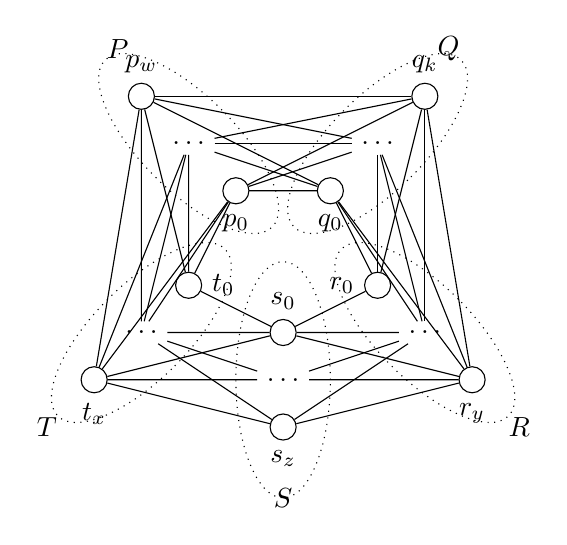
\begin{tikzpicture}[scale=0.6]
\node[draw,circle,label=$s_0$] (v4) at (-1,-4) {};
\node[circle,draw,label=right:$t_0$] (v5) at (-3,-3) {};
\node[circle,draw,label=below:$p_0$] (v1) at (-2,-1) {};
\node[circle,draw,label=below:$q_0$] (v2) at (0,-1) {};
\node[draw,circle,label=left:$r_0$] (v3) at (1,-3) {};
\node (v16) at (-3,0) {$\dots$};
\node[draw,circle,label=$p_w$] (v6) at (-4,1) {};
\node (v10) at (1,0) {$\dots$};
\node[draw,circle,label=$q_k$] (v9) at (2,1) {};
\node (v13) at (-1,-5) {$\dots$};
\node[draw,circle,label=below:$s_z$] (v12) at (-1,-6) {};
\node (v15) at (2,-4) {$\dots$};
\node[draw,circle,label=below:$r_y$] (v14) at (3,-5) {};
\node (v8) at (-4,-4) {$\dots$};
\node[draw,circle,label=below:$t_x$] (v7) at (-5,-5) {};

\draw (v1) -- (v2) -- (v3) -- (v4) -- (v5) -- (v1);
\draw  (v6) edge (v7);
\draw  (v6) edge (v8);
\draw  (v6) edge (v5);
\draw  (v6) edge (v9);
\draw  (v10) edge (v6);
\draw  (v6) edge (v2);
\draw  (v12) edge (v7);
\draw  (v13) edge (v7);
\draw  (v8) edge (v4);
\draw  (v4) edge (v7);
\draw  (v8) edge (v13);
\draw  (v8) edge (v12);
\draw  (v14) edge (v12);
\draw  (v14) edge (v13);
\draw  (v14) edge (v4);
\draw  (v15) edge (v4);
\draw  (v13) edge (v15);
\draw  (v12) edge (v15);
\draw  (v9) edge (v3);
\draw  (v9) edge (v15);
\draw  (v14) edge (v9);
\draw  (v16) edge (v9);
\draw  (v1) edge (v9);
\draw  (v10) edge (v3);
\draw  (v16) edge (v8);
\draw  (v16) edge (v7);
\draw  (v16) edge (v5);
\draw  (v16) edge (v2);
\draw  (v16) edge (v10);

\draw[dotted,rotate around={45:(-3,0)}]  (-3,0) ellipse (1 and 2.5);
\draw[dotted,rotate around={-45:(1,0)}]  (1,0) ellipse (1 and 2.5);
\draw[dotted,rotate around={-45:(-4,-4)}]  (-4,-4) ellipse (1 and 2.5);
\draw[dotted,rotate around={45:(2,-4)}]  (2,-4) ellipse (1 and 2.5);
\draw[dotted]  (-1,-5) ellipse (1 and 2.5);
\draw  (v1) edge (v7);
\draw  (v1) edge (v2);
\draw  (v14) edge (v2);
\draw  (v14) edge (v10);
\draw  (v10) edge (v15);
\draw  (v1) edge (v10);
\draw  (v1) edge (v8);
\draw  (v2) edge (v15);
\node at (-4.5,2) {$P$};
\node at (2.5,2) {$Q$};
\node at (-6,-6) {$T$};
\node at (-1,-7.5) {$S$};
\node at (4,-6) {$R$};
\end{tikzpicture}
\end{column}
\end{columns}
\end{frame}

\begin{frame}
\frametitle{Nº Envoltório}
\framesubtitle{diâmetro 2 - Maximal sem triângulo}
  \begin{columns}[T]
    \begin{column}{.7\textwidth}
\begin{lem}
\label{hs-dominante-mst}     
Seja $G$ um grafo de diâmetro 2 que não possui um $C_6$ como subgrafo induzido então existe $S^\prime \subseteq V(G)$ tal que $|S^\prime|=3$ e $H(S^\prime)$ é um conjunto dominante.
\label{prop-env-knn}
\end{lem}

\begin{coro}
    Seja $G$ um grafo de diâmetro 2 sem vértice de corte e sem $C_6$ sem corda como subgrafo então $h(G) \le 4$.
\label{teor-env-mst}
\end{coro}
    \end{column}
    \begin{column}{.3\textwidth}
    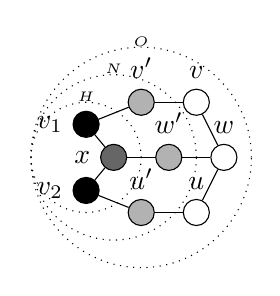
\begin{tikzpicture}[scale=0.7]
\node[circle,draw,fill=black!60,label=left:$x$] (v1) at (-1,0) {};
\node[circle,draw,fill,label=left:$v_1$] (v2) at (-1.5,0.6) {};
\node[circle,draw,fill,label=left:$v_2$] (v3) at (-1.5,-0.6) {};

\draw  (v1) edge (v2);
\draw  (v1) edge (v3);

\node[circle,draw,fill=black!30,label=$v^\prime$] (v4) at (-0.5,1) {};
\node[circle,draw,fill=black!30,label=$w^\prime$] (v9) at (0,0) {};
\node[circle,draw,fill=black!30,label=$u^\prime$] (v8) at (-0.5,-1) {};
\node[circle,draw,label=$v$] (v5) at (0.5,1) {};
\node[circle,draw,label=$w$] (v6) at (1,0) {};
\node[circle,draw,label=$u$] (v7) at (0.5,-1) {};

\draw[dotted]  (-1.5,0) ellipse (1 and 1);
\draw[dotted]  (-1,0) ellipse (1.5 and 1.5);
\draw[dotted]  (-0.5,0) ellipse (2 and 2);

\draw  (v2) edge (v4);
\draw  (v5) edge (v4);
\draw  (v5) edge (v6);
\draw  (v7) edge (v6);
\draw  (v7) edge (v8);
\draw  (v3) edge (v8);
\draw  (v6) edge (v9);
\draw  (v9) edge (v1);
\node at (-1.5,1.1) {\tiny $H$};
\node at (-1,1.6) {\tiny $N$};
\node at (-0.5,2.1) {\tiny $O$};
\end{tikzpicture}
    \end{column}
  \end{columns}
\end{frame}


\begin{frame}
\frametitle{Nº Envoltório}
\framesubtitle{diâmetro 2 - Maximal Sem Triângulo - Exemplos}
  \begin{columns}[T]
    \begin{column}{.5\textwidth}
        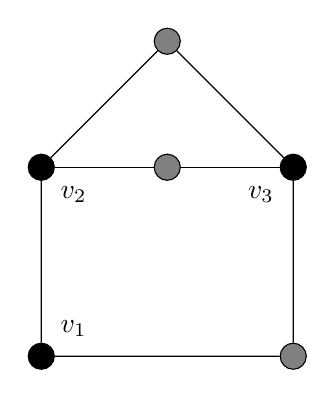
\begin{tikzpicture}[scale=0.8]
        \node[circle,draw,fill=black!50] (v9) at (0,5) {};
        \node[circle,draw,fill,label=below left:$v_3$] (v10) at (2,3) {};
        \node[circle,draw,fill=black!50] (v11) at (2,0) {};
        \node[circle,draw,fill,label=above right:$v_1$] (v12) at (-2,0) {};
        \node[circle,draw,fill,label=below right:$v_2$] (v13) at (-2,3) {};
        \node[circle,draw,fill=black!50] (v14) at (0,3) {};
        
        \draw (v9) -- (v10) -- (v11) -- (v12) -- (v13) -- (v9);
        \draw (v13) -- (v14) -- (v10);
        \end{tikzpicture}
     \end{column}
     \begin{column}{.5\textwidth}
        \centering
        \resizebox{.7\textwidth}{!}{%
            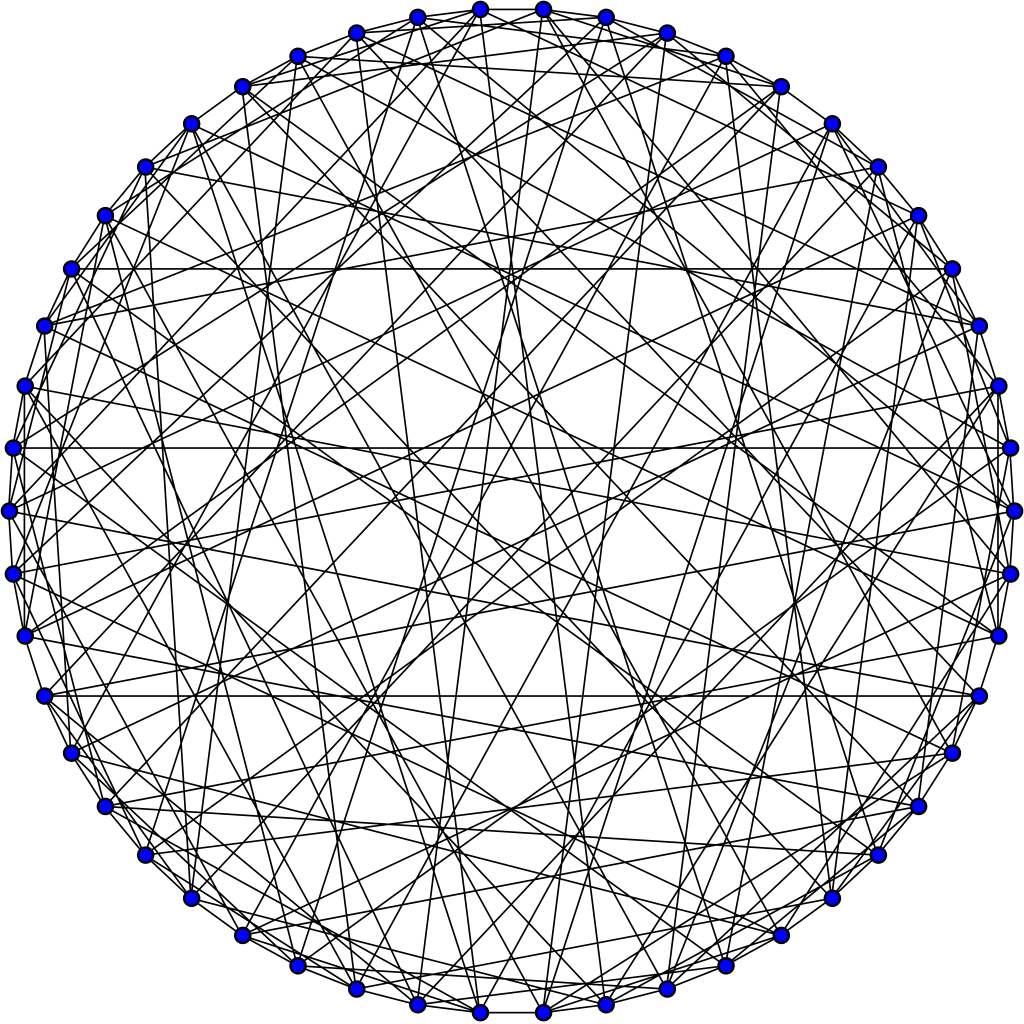
\includegraphics[scale=0.7]{img/Hoffman-Singleton_graph.png}%
        }
     \end{column}
  \end{columns}
\end{frame}   

\subsection{Fortemente Regular}

\begin{frame}
\frametitle{Nº Envoltório}
\framesubtitle{diâmetro 2 - Fortemente Regular}
  \begin{columns}[T]
    \begin{column}{.4\textwidth}
     Fortemente regular $(n,k,b,c)$:
     \begin{itemize}
         \item $n$ vértices
         \item $k$-regular
         \item $b$ vizinhos em comum todo par adjacente de vértices \item $c$ vizinhos em comum todo par não adjacente de vértices
     \end{itemize}
    \end{column}
    \begin{column}{.6\textwidth}
        \centering
        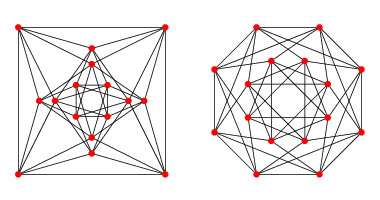
\includegraphics[scale=0.6]{img/sr.png}
    \end{column}
  \end{columns}
\end{frame}

\begin{frame}
\frametitle{Nº Envoltório}
\framesubtitle{diâmetro 2 - Fortemente Regular}

\begin{theo}
Seja $G$ um grafo fortemente regular $(n,k,b,c)$ com $c=0$ então $h(G)\le 2\omega(G)$.
\end{theo}

\begin{itemize}
    \item Se $c=0$ temos $G$ composto de componentes completas.
    \item $h(K_n)=2$ 
    \item Se $G$ é desconexo $h(G)=h(C_0)+..+h(C_n)$
\end{itemize}
\end{frame}

\begin{frame}
\frametitle{Nº Envoltório}
\framesubtitle{diâmetro 2 - Fortemente Regular e $c=0$}
\centering
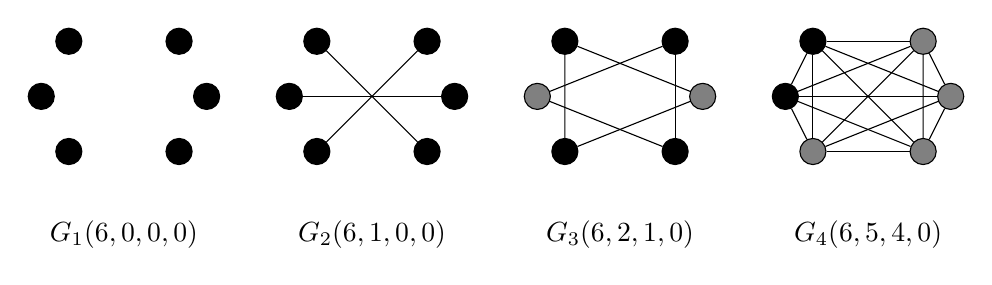
\begin{tikzpicture}[scale=0.7]
\node[circle,draw,fill] (v9) at (-19.5,-1) {};
\node[circle,draw,fill] (v5) at (-16.5,-1) {};
\node[circle,draw,fill] (v8) at (-19,-2) {};
\node[circle,draw,fill] (v6) at (-17,-2) {};
\node[circle,draw,fill] (v4) at (-17,0) {};
\node[circle,draw,fill] (v2) at (-19,0) {};
\node[circle,draw,fill] (v39) at (-15,-1) {};
\node[circle,draw,fill] (v35) at (-12,-1) {};
\node[circle,draw,fill] (v38) at (-14.5,-2) {};
\node[circle,draw,fill] (v36) at (-12.5,-2) {};
\node[circle,draw,fill] (v34) at (-12.5,0) {};
\node[circle,draw,fill] (v32) at (-14.5,0) {};
\node[circle,draw,fill=black!50] (v29) at (-10.5,-1) {};
\node[circle,draw,fill=black!50] (v25) at (-7.5,-1) {};
\node[circle,draw,fill] (v28) at (-10,-2) {};
\node[circle,draw,fill] (v26) at (-8,-2) {};
\node[circle,draw,fill] (v24) at (-8,0) {};
\node[circle,draw,fill] (v22) at (-10,0) {};
\draw  (v28) edge (v22);
\draw  (v22) edge (v25);
\draw  (v28) edge (v25);
\draw  (v29) edge (v26);
\draw  (v26) edge (v24);
\draw  (v29) edge (v24);
\draw  (v35) edge (v39);
\draw  (v36) edge (v32);
\draw  (v34) edge (v38);

\node[circle,draw,fill] (v29) at (-6,-1) {};
\node[circle,draw,fill=black!50] (v25) at (-3,-1) {};
\node[circle,draw,fill=black!50] (v28) at (-5.5,-2) {};
\node[circle,draw,fill=black!50] (v26) at (-3.5,-2) {};
\node[circle,draw,fill=black!50] (v24) at (-3.5,0) {};
\node[circle,draw,fill] (v22) at (-5.5,0) {};
\draw  (v22) edge (v24);
\draw  (v22) edge (v29);
\draw  (v22) edge (v28);
\draw  (v26) edge (v22);
\draw  (v22) edge (v25);
\draw  (v29) edge (v28);
\draw  (v28) edge (v26);
\draw  (v26) edge (v25);
\draw  (v25) edge (v24);
\draw  (v24) edge (v28);
\draw  (v24) edge (v26);
\draw  (v29) edge (v25);
\draw  (v25) edge (v28);
\draw  (v26) edge (v29);
\draw  (v24) edge (v29);

\node at (-18,-3.5) {$G_1(6,0,0,0)$};
\node at (-13.5,-3.5) {$G_2(6,1,0,0)$};
\node at (-9,-3.5) {$G_3(6,2,1,0)$};
\node at (-4.5,-3.5) {$G_4(6,5,4,0)$};
\end{tikzpicture}
\end{frame}

\begin{frame}
\frametitle{Nº Envoltório}
\framesubtitle{diâmetro 2 - Fortemente Regular}
\begin{theo}
Seja $G$ um grafo fortemente regular $(n,k,b,c)$ com $c>0$ então existe um $S'$ tal que $|S'| = \big\lceil \frac{k}{1+b} \big\rceil$ e $H(S')$ é um conjunto dominante.
\label{dom-gfr} 
\end{theo}
\begin{itemize}
    \item Se $c > 0$ temos $G$ diâmetro 2
    \item Dado $v$ podemos compor um $S^\prime \subseteq N(v)$
    \item A cada iteração um novo vértice em $S^\prime$ e $b+1$ em $H(S^\prime)$
    \item $N(v) \subseteq H(S^\prime)$ então $H(S^\prime)$ é dominante
\end{itemize}
\end{frame}

\begin{frame}
\frametitle{Nº Envoltório}
\framesubtitle{diâmetro 2 - Fortemente Regular e $c>0$}
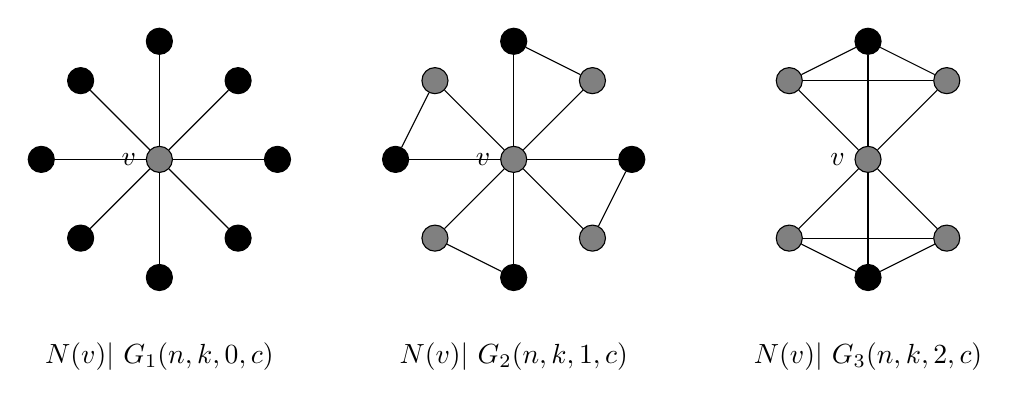
\begin{tikzpicture}
\node[circle,draw,fill=black!50,label=left:$v$] (v1) at (-13.5,-1) {};
\node[circle,draw,fill] (v3) at (-13.5,0.5) {};
\node[circle,draw,fill] (v9) at (-15,-1) {};
\node[circle,draw,fill] (v7) at (-13.5,-2.5) {};
\node[circle,draw,fill] (v5) at (-12,-1) {};
\node[circle,draw,fill] (v8) at (-14.5,-2) {};
\node[circle,draw,fill] (v6) at (-12.5,-2) {};
\node[circle,draw,fill] (v4) at (-12.5,0) {};
\node[circle,draw,fill] (v2) at (-14.5,0) {};
\draw  (v1) edge (v2);
\draw  (v1) edge (v3);
\draw  (v1) edge (v4);
\draw  (v1) edge (v5);
\draw  (v1) edge (v6);
\draw  (v7) edge (v1);
\draw  (v1) edge (v8);
\draw  (v1) edge (v9);

\node[circle,draw,fill=black!50,label=left:$v$] (v31) at (-9,-1) {};
\node[circle,draw,fill] (v33) at (-9,0.5) {};
\node[circle,draw,fill] (v39) at (-10.5,-1) {};
\node[circle,draw,fill] (v37) at (-9,-2.5) {};
\node[circle,draw,fill] (v35) at (-7.5,-1) {};
\node[circle,draw,fill=black!50] (v38) at (-10,-2) {};
\node[circle,draw,fill=black!50] (v36) at (-8,-2) {};
\node[circle,draw,fill=black!50] (v34) at (-8,0) {};
\node[circle,draw,fill=black!50] (v32) at (-10,0) {};
\draw  (v31) edge (v32);
\draw  (v31) edge (v33);
\draw  (v31) edge (v34);
\draw  (v31) edge (v35);
\draw  (v31) edge (v36);
\draw  (v37) edge (v31);
\draw  (v31) edge (v38);
\draw  (v31) edge (v39);

\node[circle,draw,fill=black!50,label=left:$v$] (v21) at (-4.5,-1) {};
\node[circle,draw,fill] (v23) at (-4.5,0.5) {};
\node[circle,draw,fill] (v27) at (-4.5,-2.5) {};
\node[circle,draw,fill=black!50] (v28) at (-5.5,-2) {};
\node[circle,draw,fill=black!50] (v26) at (-3.5,-2) {};
\node[circle,draw,fill=black!50] (v24) at (-3.5,0) {};
\node[circle,draw,fill=black!50] (v22) at (-5.5,0) {};
\draw  (v34) edge (v33);
\draw  (v36) edge (v35);
\draw  (v37) edge (v38);
\draw  (v39) edge (v32);

\node at (-13.5,-3.5) {$N(v)|$ $G_1(n,k,0,c)$};
\node at (-9,-3.5) {$N(v)|$ $G_2(n,k,1,c)$};
\node at (-4.5,-3.5) {$N(v)|$  $G_3(n,k,2,c)$};
\draw  (v22) edge (v21);
\draw  (v21) edge (v24);
\draw  (v24) edge (v22);
\draw  (v23) edge (v21);
\draw  (v22) edge (v23);
\draw  (v23) edge (v24);
\draw  (v28) edge (v21);
\draw  (v21) edge (v26);
\draw  (v27) edge (v28);
\draw  (v27) edge (v26);
\draw  (v21) edge (v27);
\draw  (v26) edge (v28);
\end{tikzpicture}
\end{frame}



\begin{frame}
\frametitle{Nº Envoltório}
\framesubtitle{diâmetro 2 - Fortemente Regular}
\begin{lem}
Considere a i-ésima iteração do algoritmo em um grafo $G$ fortemente regular $(n,k,b,c)$ com $c>0$. Se $O_i \neq \emptyset$, então $|H(S_i)|\geq (c+1) \times |H(S_{i-1})|+1$.
\label{pior-caso-hs-sr}
\end{lem}
\begin{proposition} 
No máximo haverá $i=\big \lceil \log_{c+1}(kc+1) \big \rceil$ iterações.
\end{proposition}
\begin{theo}
Seja $G$ um grafo fortemente regular e $c>0$ então $h(G) \le \big \lceil \log_{c+1}(kc+1) \big \rceil + 1$.
\end{theo}
\end{frame}



\begin{frame}
\frametitle{Nº Envoltório}
%\framesubtitle{diâmetro 2 - exemplos}
\centering
%\tiny
\resizebox{.9\textwidth}{!}{%
%\small
\begin{tabular}{r|c|c|c|c|c}
& & \multicolumn{2}{c|}{\textbf{Diâmetro 2}} 
& \multicolumn{2}{c}{\textbf{Fortemente Regular}} \\ 
\textbf{Grafo} & \textbf{h} & \textbf{Corol. 3.4}
& \textbf{Corol. 3.13} & \textbf{Corol. 3.22} & \textbf{Teor. 3.25}  \\ \hline
$C_5$ (5,2,0,1) & 3  & 3 & 3 & 3 & 3 \\ \hline
Petersen (10,3,0,1) & 3  & 4 & 3 & 4 & 3\\ \hline
Clebsch (16,5,0,2)  & 3 & 6 & 4 & 6 & 3 \\ \hline
(4,4)-Hook (16,6,2,2) & 2  & 7 & 4 & 3 & 3\\ \hline
Hoffman-Singleton (50,7,0,1) & 4 & 8 & 4 & 8 & 4 \\ \hline
Gewirtz (56,10,0,2) & 3  & 11 & 4 & 11 & 4\\ \hline
Brouwer-Haemers (81,20,1,6) & 2 & 21 & 5 & 11 & 3\\ \hline
$M_{22}$ (77,16,0,4) & 2  & 17 & 5 & 17 & 4\\ \hline
$H(2,10)$ (100,18,8,2) & 2 & 19 & 5 & 3 & 4\\ \hline
Higman-Sims (100,22,0,6) & 2  & 23 & 6 & 23 & 4\\ \hline
$1^{st}$ sub. of McLaughlin (112,30,2,10) & 2 & 113 & 8 & 5 & 3\\ \hline
Cameron (231,30,9,3) & 2  & 31 & 6 & 4 & 4 \\ \hline
Berlekamp-van L. (243,22,1,2) & 3 & 23 & 6 & 12 & 4 \\ \hline
McLaughlin (275,112,30,56)  & 2   & 113 & 8 & 5 & 3\\ \hline
Grassmann $J_2(6,2)$ (651,90,33,9) & 2 & 91 & 8 & 4 & 4 \\ \hline
G2(4) (416,100,36,20) & 2 & 101 & 8 & 4  & 3  \\ \hline
Games (729,112,1,20) & * &  113 & 8 & 57 & 4 \\ %\hline
\end{tabular}%
}
\end{frame}
